% Created 2026-07-10 vie 01:29
% Intended LaTeX compiler: pdflatex
\documentclass[11pt]{article}
\usepackage[utf8]{inputenc}
\usepackage[T1]{fontenc}
\usepackage{graphicx}
\usepackage{longtable}
\usepackage{wrapfig}
\usepackage{rotating}
\usepackage[normalem]{ulem}
\usepackage{amsmath}
\usepackage{amssymb}
\usepackage{capt-of}
\usepackage{hyperref}
\author{Grupo 7 - Grupo 8}
\date{}
\title{S11 — Sistemas de Entrada/Salida}
\hypersetup{
 pdfauthor={Grupo 7 - Grupo 8},
 pdftitle={S11 — Sistemas de Entrada/Salida},
 pdfkeywords={},
 pdfsubject={},
 pdfcreator={Emacs 27.1 (Org mode 9.3)}, 
 pdflang={Spanish}}
\usepackage{biblatex}

\begin{document}

\maketitle
\section*{Sistemas de Entrada/Salida}
\label{sec:org57bff84}
La \textbf{arquitectura de E/S} de un computador es su interfaz con el
exterior. Esta arquitectura permite una forma sistemática de controlar
su interacción con el mundo exterior a la vez que proporciona al
sistema operativo la información necesaria para para gestionar
perifericos
Para ello, existen \textbf{3 técnicas principales}:
\begin{itemize}
\item \texttt{E/S Programada}
\item \texttt{E/S mediante interrupciones}
\item \texttt{Acceso directo a memoria (DMA)}
\end{itemize}
\subsection*{Modulo de E/S}
\label{sec:org597e1c1}
Elemento clave de un computador junto al procesador y la
memoria. Permite y gestiona la comunicación entre los \textbf{periféricos} y
los \textbf{buses del sistema}

\texttt{Permite:}
\begin{itemize}
\item Realizar la interfaz entre \textbf{procesador} y \textbf{memoria} a través del bus del sistema
\item Realizar la interfaz entre uno o más \textbf{perifericos}
\end{itemize}
\subsubsection*{Funciones módulo}
\label{sec:orga05a78e}
\begin{figure}[htbp]
\centering
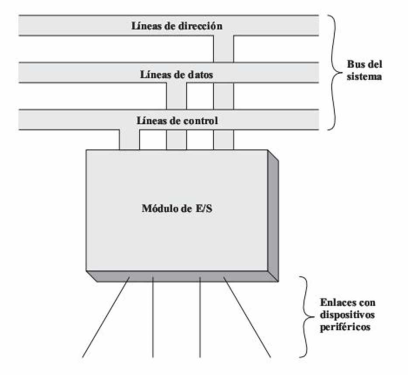
\includegraphics[width=.9\linewidth]{images/funcionesModuloES.png}
\caption{Figura 7.1. Módulo genérico E/S. Tomado de Stallings 7ma ed.}
\end{figure}
\subsubsection*{¿Por que no conectar directamente?}
\label{sec:org12affc1}
\begin{itemize}
\item Amplia \textbf{variedad} con funcionamiento variable.
\item Desincronización de \textbf{velocidades}.
\item Distintos \textbf{formatos} de datos
\end{itemize}
\begin{center}
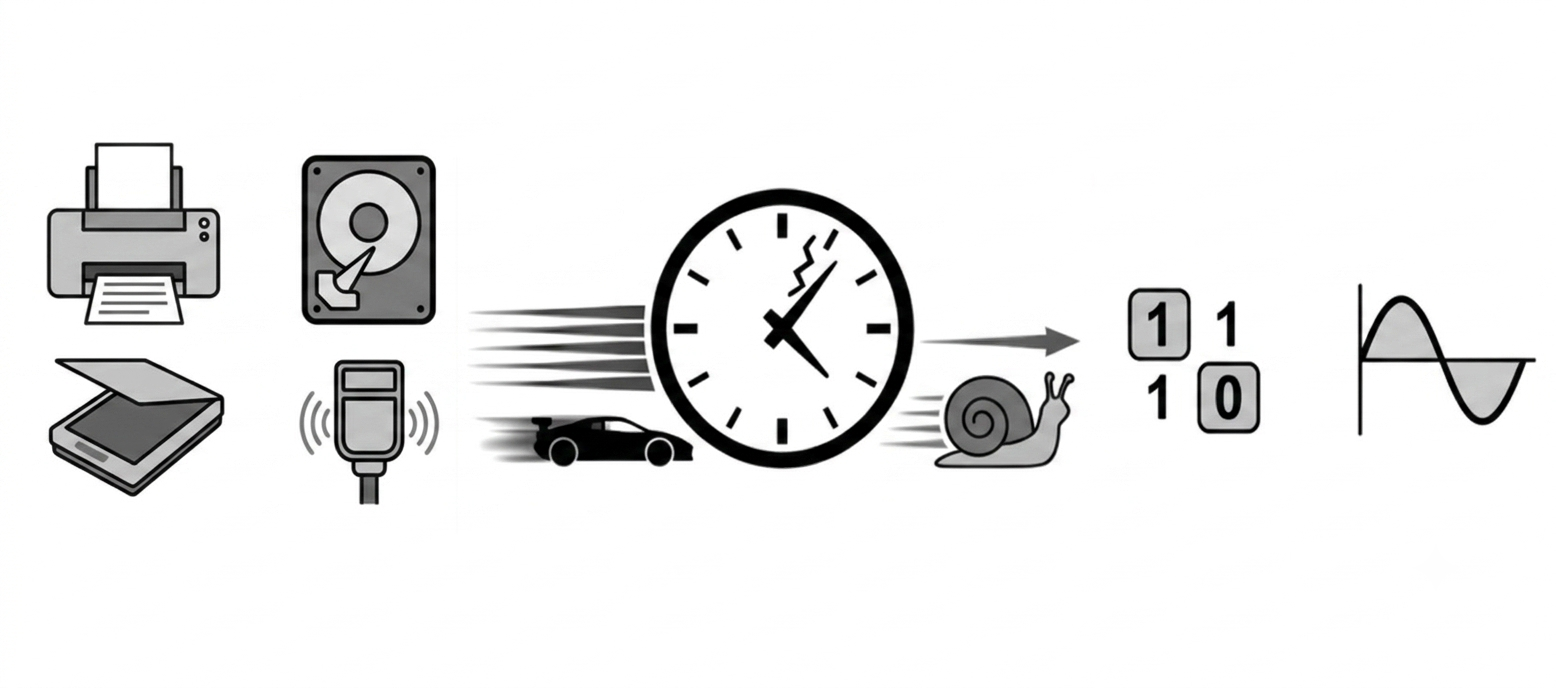
\includegraphics[width=.9\linewidth]{images/importanciaModulo.png}
\end{center}
\subsection*{Dispositivos Externos}
\label{sec:org21bbf90}
Los dispositivos externos proporcionan una forma de intercambiar datos
entre el \textbf{exterior} y el computador.

\texttt{Conexión:}
\begin{itemize}
\item Se conectan mediante un \textbf{enlace} a un módulo de E/S
\item El enlace intercambia señales de \textbf{control}, \textbf{estado} y \textbf{datos}
\item También llamados \textbf{dispositivos periféricos}
\end{itemize}
\subsubsection*{Clasificación de dispositivos externos}
\label{sec:org8a48ba9}
\begin{itemize}
\item \textbf{Interacción con humanos}: comunicación con el usuario (VDT, impresoras)
\item \textbf{Interacción con máquinas}: discos, cintas, sensores, actuadores (robótica)
\item \textbf{De comunicación}: comunicación con dispositivos remotos
\end{itemize}
\subsubsection*{Señales de control}
\label{sec:orgd9eb4d2}
Determinan la \textbf{función} que debe realizar el dispositivo
\begin{itemize}
\item \textbf{ENTRADA / LECTURA} ("INPUT" / "READ"): enviar datos al módulo de E/S
\item \textbf{SALIDA / ESCRITURA} ("OUTPUT" / "WRITE"): aceptar datos desde el módulo de E/S
\item Indicar \textbf{estado} o ejecutar una \textbf{función de control} particular
\texttt{(ej. posicionar una cabeza de disco)}
\end{itemize}
\subsubsection*{Señales de estado y datos}
\label{sec:org929dcb6}
\begin{itemize}
\item \texttt{Datos}: conjunto de bits enviados o recibidos del módulo de E/S
\item \texttt{Estado}: indica la condición del dispositivo
\begin{itemize}
\item \textbf{LISTO / NO-LISTO} ("READY/NOT-READY")
\end{itemize}
\end{itemize}
\begin{itemize}
\item \texttt{Componentes internos}
\label{sec:orgea66a69}
\begin{itemize}
\item \textbf{Lógica de control}: controla la operación según las órdenes del módulo de E/S
\item \textbf{Transductor}: convierte señales eléctricas en  otra forma de energía
\item \textbf{Buffer}: almacena temporalmente el dato en tránsito
\textbf{(tamaño típico: 8 a 16 bits)}
\end{itemize}
\end{itemize}
\subsubsection*{Diagrama de Bloques de un dispositivo externo}
\label{sec:org9964602}
\begin{figure}[htbp]
\centering
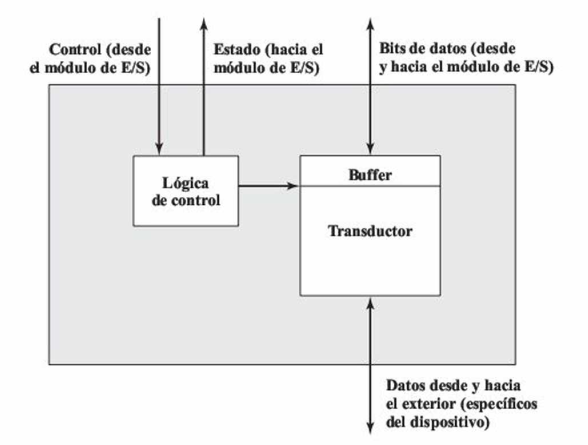
\includegraphics[width=.9\linewidth]{images/diagramaDispExt.png}
\caption{Figura 7.2. Estructura de un dispositivo externo. Tomado de Stallings 7ma ed.}
\end{figure}
\subsection*{Teclado/Monitor}
\label{sec:orgc42a384}
Forma más \textbf{común} de interacción usuario/computador
\begin{itemize}
\item \textbf{Teclado}: entrada del usuario
\item \textbf{Monitor}: muestra entrada y datos del computador
\item Unidad básica de intercambio: el \textbf{carácter}
\end{itemize}
\begin{itemize}
\item \texttt{Flujo de la señal}
\label{sec:orga07ecb3}
\begin{itemize}
\item \textbf{Entrada}: tecla → transductor → código IRA → módulo de E/S
\item \textbf{Salida}: módulo de E/S → código IRA → transductor → carácter en pantalla
\end{itemize}
\end{itemize}
\subsubsection*{Código IRA}
\label{sec:org6d669c5}
\begin{itemize}
\item \textbf{7 bits} → 128 caracteres posibles \texttt{(similar a ASCII)}
\item Dos tipos: \textbf{imprimibles} (letras, números) y \textbf{de control} (ej. retorno de carro)
\item Ejemplo: la letra \textbf{K} = \texttt{1001011}
\end{itemize}
\subsubsection*{Tabla código ASCII}
\label{sec:org8e73773}
\begin{figure}[htbp]
\centering
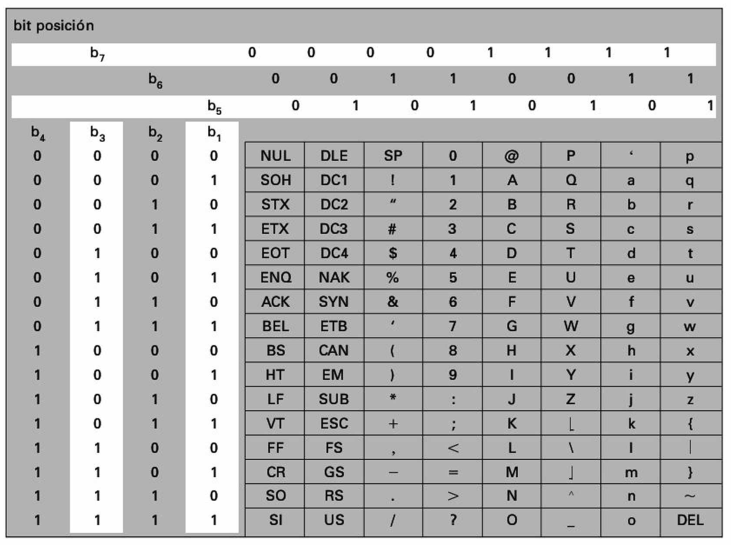
\includegraphics[width=.9\linewidth]{images/codigoASCII.png}
\caption{Figura 7.3. Tabla del código ASCII. Tomado de Stallings 7ma ed.}
\end{figure}
\subsection*{Controlador de Disco (Disk Drive)}
\label{sec:org7ce5b15}
Contiene la electrónica para:
\begin{itemize}
\item Intercambiar señales de \textbf{datos}, \textbf{control} y \textbf{estado} con el módulo de E/S
\item Controlar el mecanismo de \textbf{lectura/escritura} del disco
\end{itemize}
\begin{itemize}
\item \texttt{Tipos de disco}
\label{sec:org2910332}
\begin{itemize}
\item \textbf{Cabeza fija}: el transductor convierte patrones magnéticos ↔ bits del buffer
\item \textbf{Cabeza móvil}: además mueve el brazo \textbf{radialmente} sobre la superficie del disco
\end{itemize}
\end{itemize}
\section*{Módulos de E/S}
\label{sec:orgbb7ea34}

\subsection*{Funciones del módulo de E/S}
\label{sec:orgd0c7d5c}

Las principales funciones de un módulo de E/S son:

\begin{itemize}
\item Control y temporización
\item Comunicación con el procesador
\item Comunicación con el dispositivo
\item Buffer de datos
\item Detección de errores
\end{itemize}
\subsection*{Comunicación con el procesador}
\label{sec:org0fbcf51}

\begin{enumerate}
\item El procesador interroga al módulo de E/S
\item El módulo de E/S devuelve el estado del dispositivo
\item El procesador solicita la transferencia del dato
\item El módulo obtiene un dato
\item Los datos se transfieren al procesador
\end{enumerate}

\textbf{La comunicación con el procesador implica:}
\begin{itemize}
\item Decodificación de órdenes  -Información de Estado
\item Datos                      -
\end{itemize}
\subsection*{Almacenamiento Temporal y detección de errores}
\label{sec:org502c80a}

\textbf{Buffer de datos}

\begin{itemize}
\item Compensa diferencias de velocidad
\item Almacena temporalmente los datos
\item Sincroniza CPU y periféricos
\end{itemize}

\textbf{Detección de errores}

\begin{itemize}
\item Fallos del dispositivo
\item Errores de transmisión
\item Bit de paridad
\end{itemize}
\subsection*{Estructura de un módulo de E/S}
\label{sec:orgf91ca8e}

\begin{figure}[htbp]
\centering
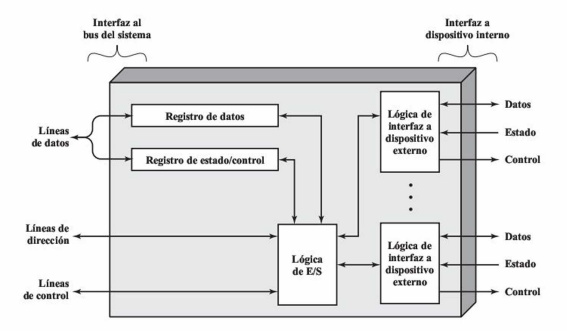
\includegraphics[width=.9\linewidth]{images/BloquesES.png}
\caption{Diagrama de bloques de un módulo de E/S}
\end{figure}
\section*{E/S Programada}
\label{sec:org5a68bf2}

\subsection*{E/S Programada}
\label{sec:orga97a2d5}

La CPU controla completamente la operación de E/S.

\begin{itemize}
\item Envía una orden al módulo de E/S
\item Consulta continuamente el estado
\item Espera hasta finalizar la operación
\item No utiliza interrupciones
\end{itemize}

Polling (espera activa)
\subsection*{Órdenes de E/S}
\label{sec:org8640256}

\begin{center}
\begin{tabular}{ll}
Orden & Función\\
\hline
Control & Activa o configura el dispositivo\\
Test & Consulta el estado\\
Lectura & Obtiene datos del dispositivo\\
Escritura & Envía datos al dispositivo\\
\end{tabular}
\end{center}
\subsection*{Funcionamiento de la E/S Programada}
\label{sec:org3cef0f9}
\begin{figure}[htbp]
\centering
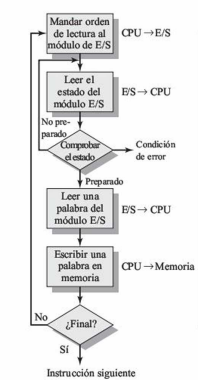
\includegraphics[width=.9\linewidth]{images/DiagramaFlujo.png}
\caption{Flujo de la E/S Programada}
\end{figure}

\begin{itemize}
\item La CPU verifica el estado del dispositivo, si no está listo continúa esperando
\end{itemize}
\section*{E/S mediante Interrupción}
\label{sec:org499affe}

El módulo de E/S \textbf{interrumpe} al procesador cuando tiene el dato listo.

\begin{itemize}
\item El CPU \textbf{no espera} — continúa con otra tarea
\item El dispositivo \textbf{avisa} cuando está listo
\item Se evita el \emph{polling} (espera activa)
\end{itemize}
\subsection*{E/S mediante Interrupción (11, 280) (7, 243)}
\label{sec:orgc448630}

\textbf{Diferencia clave frente a E/S Programada:}

\begin{center}
\begin{tabular}{ll}
E/S Programada & E/S por Interrupciones\\
\hline
CPU pregunta sin parar & Dispositivo avisa al CPU\\
CPU bloqueado & CPU libre para otras tareas\\
Espera activa & Espera pasiva\\
\end{tabular}
\end{center}
\subsection*{Procesamiento de la Interrupción}
\label{sec:org69e69c5}

\textbf{Hardware:}

\begin{enumerate}
\item Dispositivo envía señal de interrupción
\item CPU termina la instrucción en curso
\item CPU guarda \textbf{PC} y \textbf{PSW} en la pila
\item CPU salta a la rutina de interrupción
\end{enumerate}

\textbf{Software:}

\begin{enumerate}
\item Se guardan los registros del procesador
\item Se procesa la interrupción
\item Se restauran registros, PC y PSW
\item El programa original continúa
\end{enumerate}
\subsection*{Problemas de diseño}
\label{sec:org78aa8fc}
\textbf{¿Cómo saber qué dispositivo interrumpió?}

\begin{itemize}
\item Múltiples líneas de interrupción
\item Consulta de software (\emph{polling})
\item Conexión en cadena (\emph{daisy chain})
\item Arbitraje de bus
\end{itemize}

\textbf{¿A cuál atender si llegan varias a la vez?}

\begin{itemize}
\item Se asignan \textbf{niveles de prioridad} a cada dispositivo
\end{itemize}
\section*{Acceso directo a Memoria DMA}
\label{sec:org4bd0ec6}

\begin{center}
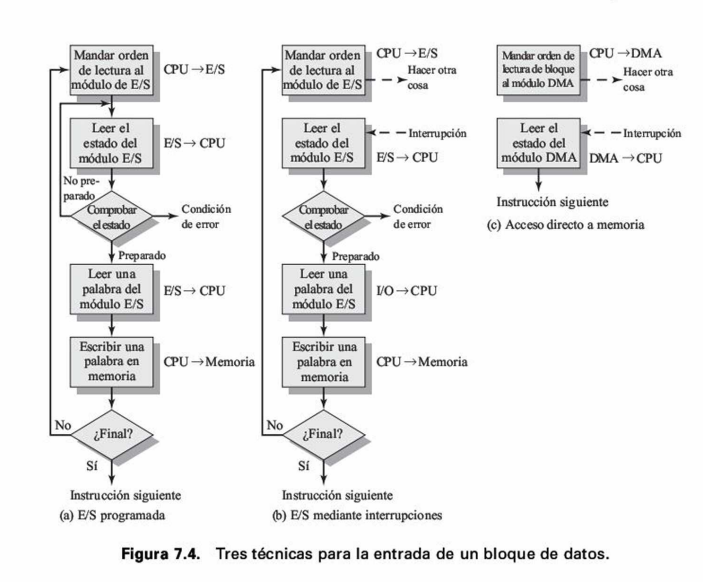
\includegraphics[width=.9\linewidth]{images/figura-7.4.png}
\end{center}
\subsection*{Funcionalidad de DMA}
\label{sec:org7a2229c}
El \textbf{\textbf{DMA (Direct Memory Access)}} es un módulo que permite realizar
transferencias de datos entre memoria y dispositivos de E/S sin la
intervención constante del procesador.

Para ello:
\begin{itemize}
\item Solicita el control del bus del sistema al CPU.
\item Realiza la transferencia de datos.
\item Libera el bus cuando termina.
\end{itemize}

En \textbf{Cycle Stealing}, el DMA utiliza temporalmente el bus.
\subsection*{El procesador no se detiene igual que con una interrupción}
\label{sec:org74d513e}
\begin{itemize}
\item EL DMA detiene al procesador por un ciclo de bus, no lo interrumpe
\item No guarda contexto.
\end{itemize}
\begin{center}
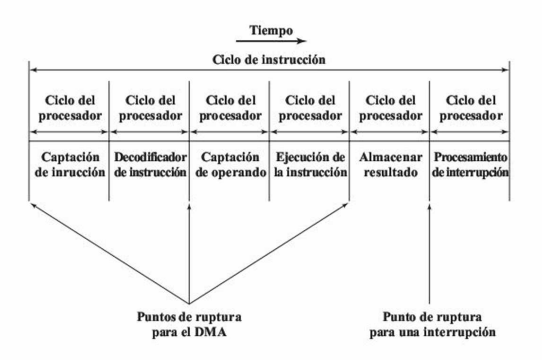
\includegraphics[width=.9\linewidth]{images/figura_7.12.png}
\end{center}
\subsection*{Configuraciones del DMA en el sistema}
\label{sec:org25f29fc}
\begin{itemize}
\item \textbf{Bus único}: Todos comparten el mismo bus
\item \textbf{DMA - E/S integrados:} El DMA se conecta directamente a
los periféricos
\item \textbf{Bus E/S propio:} El DMA tiene un bus exclusivo para los
dispositivos
\end{itemize}
\subsection*{Configuraciones del DMA en el sistema}
\label{sec:org47fde26}
\begin{center}
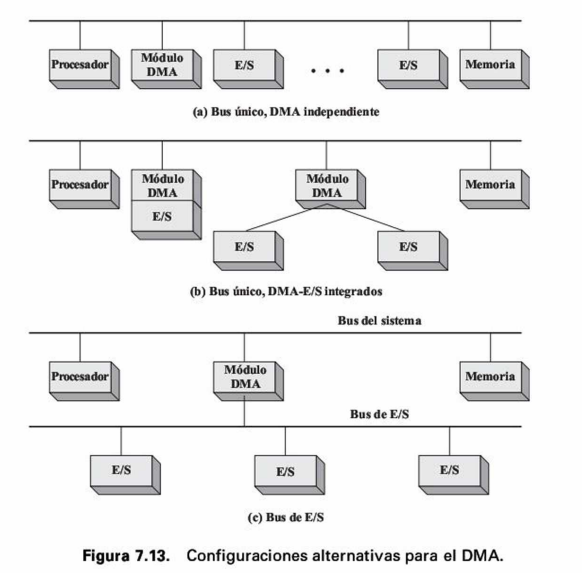
\includegraphics[width=.9\linewidth]{images/figura_7.13.png}
\end{center}
\subsection*{Controlador Intel 8237 A}
\label{sec:org36989e3}
\begin{itemize}
\item Controlador de DMA de Intel
\item Le da acceso directo a la memoria DRAM en computadores con
procesadores 80x86
\item No almacena ni transporta, solo genera señales de control
\item Llamado también controlador fly-by o de vuelo.
\end{itemize}
\begin{center}
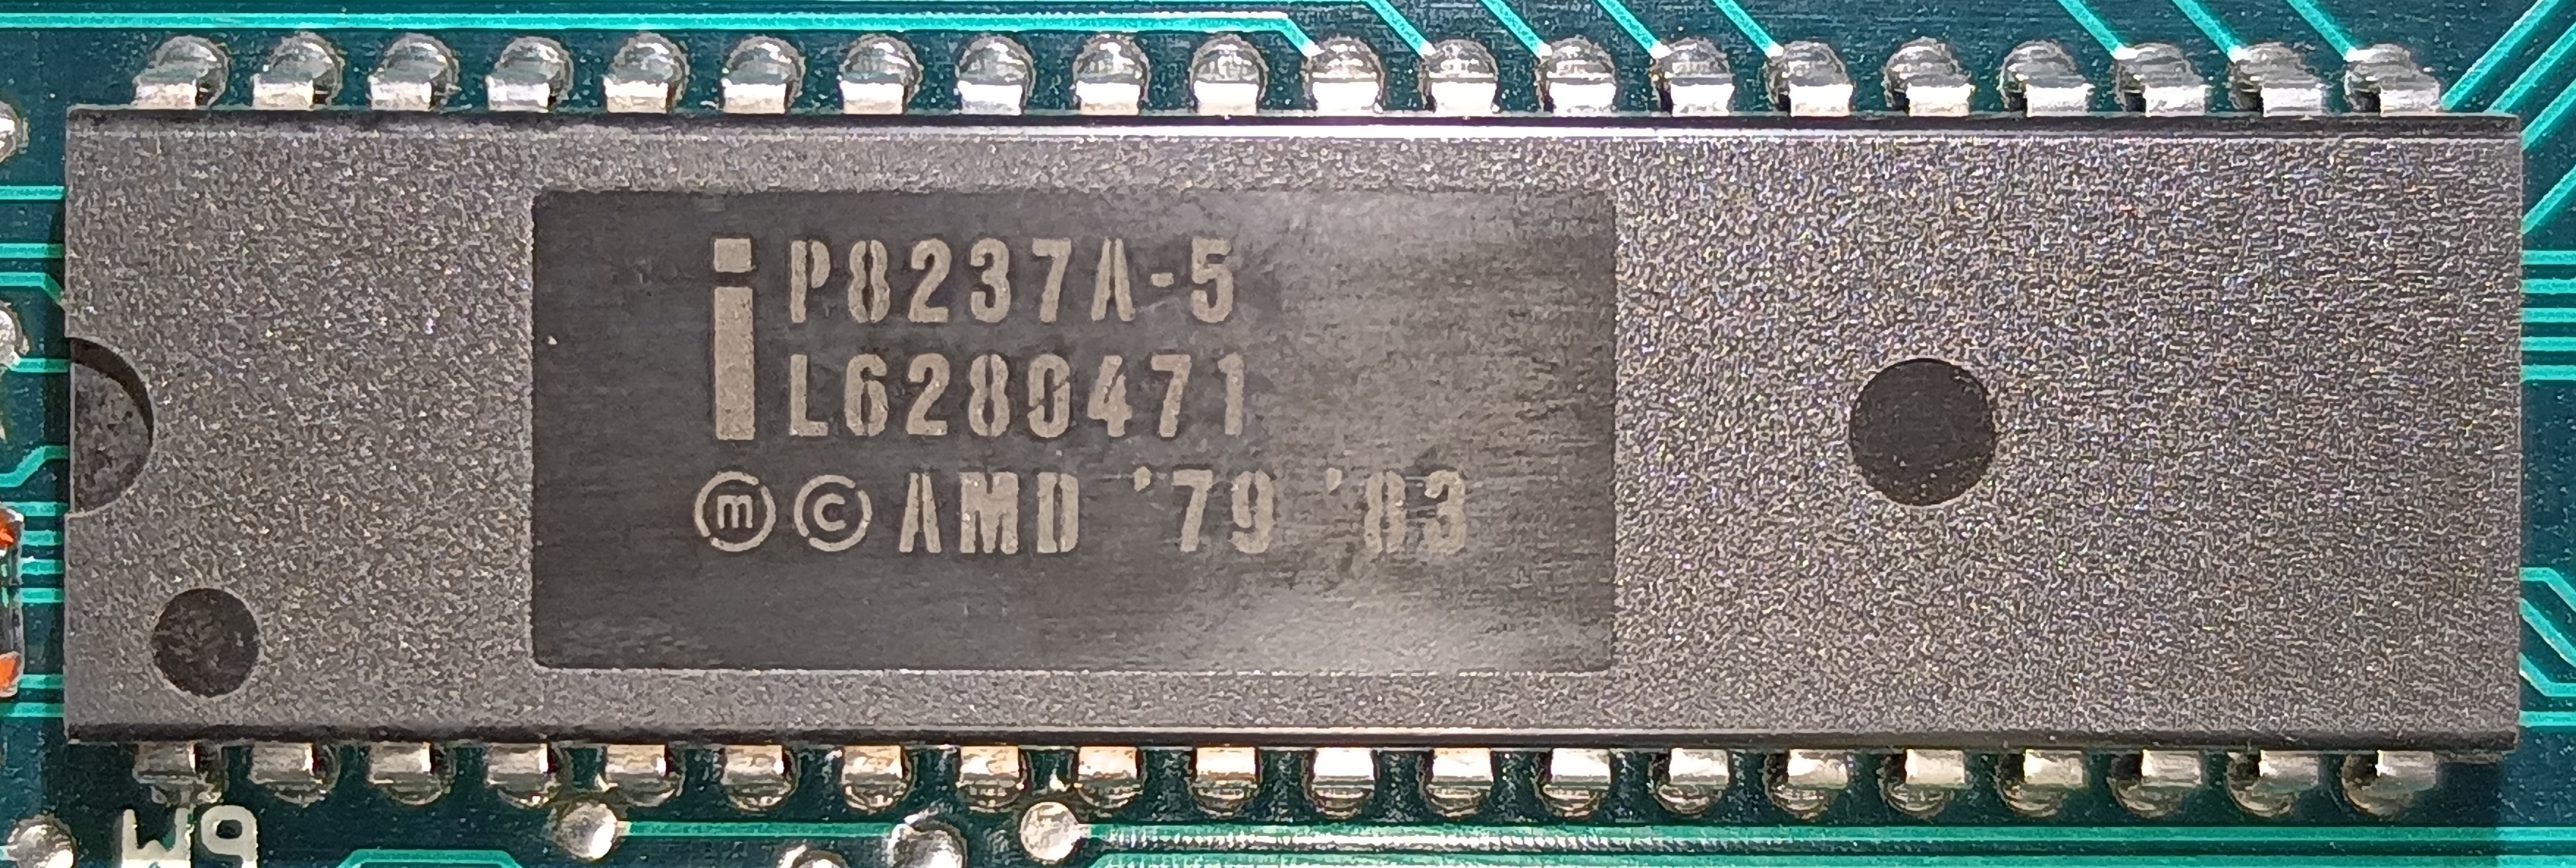
\includegraphics[width=.9\linewidth]{images/inte.jpg}
\end{center}
\subsection*{Señales}
\label{sec:orge2216ef}
\textbf{Señales HOLD/HOLAD (Controlaodr del DMA - CPU)}
\begin{itemize}
\item \textbf{HOLD}: DMA pide el bus
\item \textbf{HLDA(Hold Acknowledge)}:Indica que se pueden usar los buses
\end{itemize}
\textbf{Señales DREQ/DACK (Periférico - Controlador del DMA})
-\textbf{DREQ (DMA Request)}:El periférico solicita el DMA
-\textbf{DACK (DMA Acknowledge)}: El DMA indica que se van a empezar a
transferir datos
\subsection*{Secuencia paso a paso}
\label{sec:org0d896ff}
\begin{enumerate}
\item Periférico activa \textbf{DREQ}
\item Controlador activa \textbf{HRQ} (Hold request) hacia la CPU
\item CPU termina su ciclo de bus y responde con \textbf{HLDA}
\item Controlador activa \textbf{DACK}
\item Transfiere byte a byte (MEMR/IOW), decrementando el contador
\item Al llegar a cero, desactiva el HRQ y devuelve el bus
\end{enumerate}
\subsection*{Canales y registros del 8237 a}
\label{sec:orgaea20de}
Dispone de cuatro canales de DMA independientes numerados del 0 al 3
Dispone de 5 registros de control para programar y controlar la
operación del DMA en cada uno de los canales.
\begin{center}
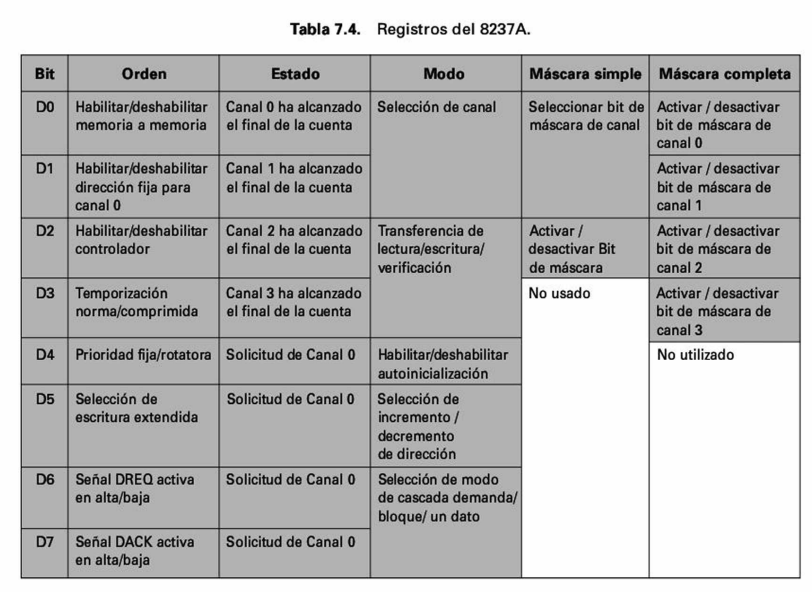
\includegraphics[width=.9\linewidth]{images/tabla 7.4.png}
\end{center}
\section*{G8 — Canales y Procesadores de E/S}
\label{sec:orgdb341df}
\subsection*{Canales y Procesadores de E/S}
\label{sec:org6cf97fe}
\subsection*{Evolución de las funciones E/S}
\label{sec:org96bb021}
\subsection*{Características de los canales E/S}
\label{sec:org6579748}
\section*{G8 — Estándares de interconexión externa}
\label{sec:org60ecc66}
\subsection*{USB}
\label{sec:org9f1939e}
\subsection*{FireWire}
\label{sec:org71860d2}
\subsection*{SCSI}
\label{sec:org430f017}
\subsection*{Thunderbolt}
\label{sec:org626a14a}
\subsection*{SATA}
\label{sec:org3cc51ed}
\subsection*{Ethernet}
\label{sec:org495bfb8}
\subsection*{Wi-Fi}
\label{sec:org21a49ff}

\printbibliography
\end{document}
